%
% File emnlp2018.tex
%
%% Based on the style files for EMNLP 2018, which were
%% Based on the style files for ACL 2018, which were
%% Based on the style files for ACL-2015, with some improvements
%%  taken from the NAACL-2016 style
%% Based on the style files for ACL-2014, which were, in turn,
%% based on ACL-2013, ACL-2012, ACL-2011, ACL-2010, ACL-IJCNLP-2009,
%% EACL-2009, IJCNLP-2008...
%% Based on the style files for EACL 2006 by 
%%e.agirre@ehu.es or Sergi.Balari@uab.es
%% and that of ACL 08 by Joakim Nivre and Noah Smith

\documentclass[11pt,a4paper]{article}
\usepackage[hyperref]{emnlp2018}
\usepackage{times}
\usepackage{latexsym}
\usepackage{graphicx, amsmath, verbatim, booktabs}
\usepackage{cite}

%\usepackage{url}

\aclfinalcopy % Uncomment this line for the final submission

%\setlength\titlebox{5cm}
% You can expand the titlebox if you need extra space
% to show all the authors. Please do not make the titlebox
% smaller than 5cm (the original size); we will check this
% in the camera-ready version and ask you to change it back.

\newcommand\BibTeX{B{\sc ib}\TeX}
\newcommand\confname{EMNLP 2018}
\newcommand\conforg{SIGDAT}


\title{Document-Level Entity-to-Entity Sentiment Analysis \\ with LSTM-Based Models}

\author{Belinda Li \\
  Paul G. Allen School of Computer Science \& Engineering \\
  Univ. of Washington, Seattle, WA \\
  %{\tt lib49@cs.washington.edu}
  \\}

\date{}

\begin{document}
\maketitle
\begin{abstract}
  Most work in fine-grained sentiment analysis is focused on predicting sentiment from within a sentence.
  These sentences usually involve only a single sentiment being expressed from one holder to one target.
  Instead, we aim to perform document-level entity-to-entity sentiment analysis, whereby we predict various sentiments among all entities at the document level.
  These sentiments may be expressed within or across sentences, and different entities may hold different sentiments towards each other.
  Sentence-level models which predict a single sentiment do not generalize well to our task, as they are unable to account for cross-sentence sentiments.
  Therefore, we propose two novel LSTM-based architectures for this task, and show that both models outperform sentence-level baselines.
%  Our model considers all entities within the document as possible holders and targets, and classifying the sentiment of each (document, holder entity, target entity) triple. 
  Surprisingly, however, we find that our models do not outperform state-of-the-art SVM-based models.
  In particular, we find that LSTM-based models have difficulty classifying entities which express no sentiment towards each other, a limitation which accounts for 60-80\% of its mistakes on the development set.
\end{abstract}

\section{Introduction}
% Sentiment analysis is a multifaceted task, involving the identification of opinion polarities, opinion holders, and opinion targets.
% characterize the polarity of that opinion and the strength of that opinion.
Historically, research in sentiment analysis has focused on finding the overall sentiment of a short span of text, like tweets \citep{DBLP:journals/corr/MohammadKZ13, DBLP:journals/corr/abs-1804-00482, DBLP:journals/corr/abs-1803-08910}, product reviews \citep{Fang2015}, or movie reviews \citep{DBLP:journals/corr/cs-CL-0409058}.
However, in recent years, there has been a shift towards more fine-grained opinion mining.
Not only is the overall sentiment of a piece of text determined, but the opinion holder and target are also identified.
This allows for a much more nuanced understanding of the sentiments expressed within a text.
\par Much of the work in fine-grained sentiment analysis has focused on classifying sentiments within a single sentence, containing a single entity pair mention.
However, sentiments are expressed in all types of texts, many of which contain multiple entity pairs and multiple mentions of each entity.
News articles in particular often encode complex networks of opinions amongst a multitude of entities.
Many of these sentiments are expressed across sentences and cannot be captured by sentence-level models.
Take this article from Xinhua News Agency as an example:
\begin{figure} \label{fig:intro}
\centering
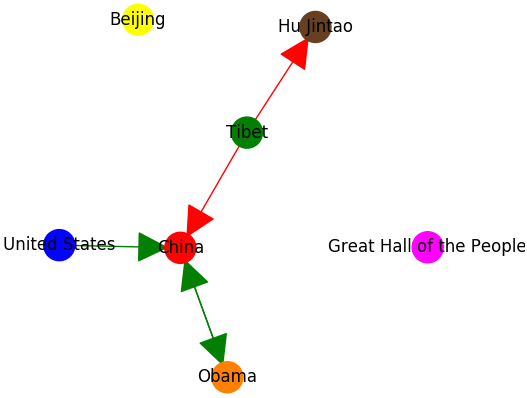
\includegraphics[scale=0.5]{example_article.png}
\caption{Graph showing the network of sentiments expressed amongst various entities in the Xinhua News Agency article. Arrows are directed from opinion holder to opinion target. \textcolor{red}{Red} arrows indicate negative sentiment and \textcolor[rgb]{0, 0.5, 0}{green} arrows indicate positive sentiment. Disconnected nodes represent entities that are present in the text, but do not participate in any sentiment relations, either as opinion holders or opinion targets.}
\end{figure}
\begin{quote}
URGENT: \textcolor[rgb]{1, 0.5, 0}{\textbf{Obama}} says \textcolor[rgb]{0, 0, 1}{\textbf{U.S.}} recognizes \textcolor[rgb]{0, 0.5, 0}{\textbf{\textcolor[rgb]{0, 0.5, 0}{\textbf{Tibet}} as part of \textcolor[rgb]{1, 0, 0}{\textbf{China}}}}. \textcolor[rgb]{0, 0, 1}{\textbf{United States}} President \textcolor[rgb]{1, 0.5, 0}{\textbf{Barack Obama}} Tuesday said the \textcolor[rgb]{0, 0, 1}{\textbf{U.S.}} government recognizes that \textcolor[rgb]{0, 0.5, 0}{\textbf{Tibet}} is \textcolor[rgb]{0, 0.5, 0}{\textbf{part of the \textcolor[rgb]{1, 0, 0}{\textbf{People's Republic of China}}}}. He also said that \textcolor[rgb]{0, 0, 1}{\textbf{the \textcolor[rgb]{0, 0, 1}{\textbf{United States}}}} supports the early resumption of dialogue between the \textcolor[rgb]{1, 0, 0}{\textbf{Chinese}} government and representatives of the Dalai Lama to resolve any concerns and differences that the two sides may have. ``\textcolor[rgb]{0, 0, 1}{\textbf{The \textcolor[rgb]{0, 0, 1}{\textbf{United States}}}} respects the sovereignty and territorial integrity of \textcolor[rgb]{1, 0, 0}{\textbf{China}},'' \textcolor[rgb]{1, 0.5, 0}{\textbf{Obama}} said at a joint press conference with \textcolor[rgb]{1, 0, 0}{\textbf{Chinese}} President \textcolor[rgb]{0.4, 0.25, 0.13}{\textbf{Hu Jintao}} at \textcolor[rgb]{1, 1, 0}{\textbf{Beijing}}'s \textcolor[rgb]{1, 0, 1}{\textbf{Great Hall of the People}}.
\end{quote}
Five sentiments have been labelled within this article:
\begin{enumerate}
\item \textcolor[rgb]{1, 0.5, 0}{\textbf{Obama}} is \textcolor[rgb]{0, 0.5, 0}{positive} towards \textcolor[rgb]{1, 0, 0}{\textbf{China}}
\item \textcolor[rgb]{0, 0, 1}{\textbf{United States}} is \textcolor[rgb]{0, 0.5, 0}{positive} towards \textcolor[rgb]{1, 0, 0}{\textbf{China}}
\item \textcolor[rgb]{1, 0, 0}{\textbf{China}} is \textcolor[rgb]{0, 0.5, 0}{positive} towards \textcolor[rgb]{1, 0.5, 0}{\textbf{Obama}}
\item \textcolor[rgb]{0, 0.5, 0}{\textbf{Tibet}} is \textcolor[rgb]{1, 0, 0}{negative} towards \textcolor[rgb]{1, 0, 0}{\textbf{China}}
\item \textcolor[rgb]{0, 0.5, 0}{\textbf{Tibet}} is \textcolor[rgb]{1, 0, 0}{negative} towards \textcolor[rgb]{0.4, 0.25, 0.13}{\textbf{Hu Jintao}}
\end{enumerate}
The fifth sentiment, in particular, involves entities that are never even mentioned in the same sentence, requiring cross-sentence reasoning.
\par We formulate our task of entity-to-entity sentiment analysis in a pipelined manner.
In the first step, all entities within a document are extracted and labelled.
Co-reference resolution is performed to identify all mentions of each entity.
In the second step, we consider each pair of entities and classify their sentiment relationship into three possible types: positive, negative, or none.
This is opposed to previous approaches which first identified the sentiment of a text, and then the holder and target of that sentiment \citep{Kim:2006}.
Such an approach works well for short texts expressing a single main sentiment, but works less well for long documents containing multiple sentiment relations.
As strong NER and coreference \citep{Lee:17} models exist already, we focus the bulk of our work on the second task, allocating the first task to preprocessing.
We propose two novel neural architectures for this task, and show that it outperforms sentence-level baselines.

\section{Data}
\begin{table*}[!t]
\centering
\begin{tabular}{| l | r | r | r | r | r | r |}
\hline
 & & Entities & & & & \\
Dataset & Docs & / Doc & Neg & None & Pos & \% None \\ \hline \hline
train-original & 897 & 2.63 & 648 & 815 & 355 & 44.8 \\
train-new & 949	 & 8.98 & 973 & 11306 & 1013 & 85.1 \\
dev-tune & 38 & 8.82 & 158 & 2349 & 365 & 81.8 \\
dev-eval& 37 & 9.08 & 174 & 2454 & 404 & 80.9 \\
test-KBP & 79 & 9.25 & 437 & 5459 & 718 & 82.5 \\
test-MPQA & 54 & 11.72 & 521 & 6464 & 625 & 84.9 \\
\hline
\end{tabular}
\caption{\label{tab:data} Dataset statistics. For each dataset, shows the total number of articles, the average number of entities within each article, the total number of negative pairs, none pairs, positive pairs, and the percentage of all pairs that are none.}
\end{table*}

We use five datasets from \citet{Choi:16} for training, development, and testing.
These datasets contain the text of a document, and annotations for each entity pair in the document.
% that are densely annotated at the entity-level, but not the mention-level.
The training set (``train-original") comprises of news articles from the Gigaword corpus\footnote{LDC2014E13:TAC2014KBP English Corpus}.
Human-annotated labels were generated for this set via crowdsourcing.
The KBP set, derived from the KBP competition, was used for development and testing.
Gold-standard annotations for this set were supplemented with human annotations to create labels between all entity pairs.
The KBP set was then split, with 50\% of the documents being used for development and 50\% for testing (``test-KBP"). 
The development set itself was also split, as 50\% of the development data was used for hyper-parameter tuning (``dev-tune") and the rest for evaluation (``dev-eval").
A second test set (``test-MPQA") was also used, derived from densely-labelled MPQA dataset.

\subsection{Training Data}
\par The distribution of the original training set does not mimic that of the development and test sets, most notably due to its lack of ``none" labels.
Such domain differences can problematic for deep neural networks in NLP \citep{Mou:16}.
Therefore, to optimize our model's performance, we make two changes to the training set.
First, we incorporate dev-tune into our training set, using dev-eval for both hyper-parameter tuning and evaluation.
As dev-tune, dev-eval, and test-KBP are all derived from the same corpus, their distributions should match.
Second, we supplement the training data with weakly generated ``none" pairs.
As the original training set did not have annotations between all pairs of entities within a document (whereas all the other dev and test sets did), we can generate new examples by finding un-labelled pairs and assuming those pairs hold no sentiment.
We then randomly select 10\% of the newly generated pairs and add them to the training data, which was sufficient to increase the proportion of ``none" pairs in the training data to 85\%, comparable to the 80-85\% found in the development and test sets.
Table \ref{tab:data} shows that the distribution of the new training dataset (``train-new") is now much closer to that of the development and test sets.
% The statistics for the old and new training data, as well as the development and test data, are fond in table \ref{tab:data}

\subsection{Preprocessing}
We use preprocessed data from \citet{Choi:16}, discarding part-of-speech tags and dependency paths which are not used by our model.
Instead, the preprocessing pipeline for our model consists of only three steps: tokenization, NER, and co-reference resolution.
Stanford CoreNLP \citep{Manning:14} was used for all three steps.
Following NER, entities of type date, duration, money, time, and number were discarded, as they do not tend to participate in sentiment relations.
Coreference resolution was performed on the remaining entities to isolate all mentions of the entity.
% Several heuristics were applied to identify named entities which refer to the same entity, and all mentions of those entities were merged into a single co-reference chain.

\section{Models}
We formulate our task by considering all entities within a document as potential holders and targets of sentiments. If there are $E$ entities in the document, then we consider $E(E - 1)$ holder-target pairs for the document.
For each pair, we classify its sentiment into one of $\{$positive$,$ negative$,$ none$\}$.
% whether a sentiment exists from the holder to the target, and whether the sentiment is positive or negative.
We explore two different neural models for this task.

\subsection{Attentive BiLSTM (``ABL")}

\noindent\textbf{Inputs.}
We concatenate three sets of embeddings to represent each token $x_t$: word embeddings ($w_t$), learned polarity embeddings ($p_t$), and learned holder-target embeddings ($e_t$):
	$$x_t = [w_t, p_t, e_t]$$
Pre-trained GloVe vectors \citep{Pennington:14} are used for word embeddings.
We also explicitly encode the polarity of known subjectivity clues (words which may be used in a positive or negative context) by appending embeddings for its polarity.
We use a pre-existing lexicon of over 8000 subjectivity clues from \citet{Wilson:05} and learn different embeddings for positive, negative, and neutral words.
Finally, our model architecture has no notion of which tokens are holders and which are targets as it treats all tokens the same.
Thus, we rely on a holder-target embedding to encode whether each token is part of a holder or target span.

\noindent\textbf{LSTM.}
We feed each embedded token $x_t$ into a bidirectional LSTM to encode it within its context.
\begin{align*}
f_{t, \delta} & = \sigma(\textbf{W}_f [x_t, h_{t + \delta, \delta}] + b_i) \\
o_{t, \delta} & = \sigma(\textbf{W}_o[x_t, h_{t + \delta,\delta}] + b_o) \\
\tilde{c}_{t, \delta} & = \tanh(\textbf{W}_c[x_t, h_{t + \delta, \delta}] + b_c) \\
c_{t, \delta} & = f_{t, \delta}\circ \tilde{c}_{t, \delta} + (1 - f_{t, \delta})\circ c_{t + \delta, \delta} \\
h_{t, \delta} & = o_{t, \delta}\circ \tanh(c_{t,\delta}) \\
x^*_t & = [h_{t, 1}, h_{t, -1}]
\end{align*}
whereby $\delta = \{1, -1\}$ indicates directionality of the LSTM.
The final representation of the token $x_t^*$ is a concatenation of the output from the forward LSTM and that from the backward LSTM.

\noindent\textbf{Attention.}
We use an attentional mechanism over all contextually-encoded tokens $x_t^*\in \{x_0^*, \dots, x_T^*\}$ to extract a final sentiment score $s_{i, j}$ from holder $i$ to target $j$.
\begin{align*}
\alpha_{t} & = \textbf{W} \cdot x^*_t \\
a_{i, j, t} & = \frac{\exp{(\alpha_t)}}{\sum^{T}_{k=0} \exp{(\alpha_k)}} \\
s_{i, j} & = \sum^{T}_{t = 0} a_{i, j, t}\cdot x_t^*
\end{align*}

\noindent\textbf{Hyperparameters.}
The GloVe embeddings, learned polarity embeddings, and learned holder-target embeddings are 50-dimensional each.
For the biLSTM, we use 2 stacked layers and a hidden dimension of 50. We apply a dropout to the hidden layer of the LSTM with probability 0.2.
For training, we optimize the model using Adam with $\alpha$ = 1e-3, $\beta_1$ = 0.9, $\beta_2$ = 0.999, $\epsilon$ = 1e-8. We use a batch size of 50, training up to 15 epochs, with epoch 6 being selected as the optimal epoch based on development set performance.

\begin{figure} \label{fig:model1}
\centering
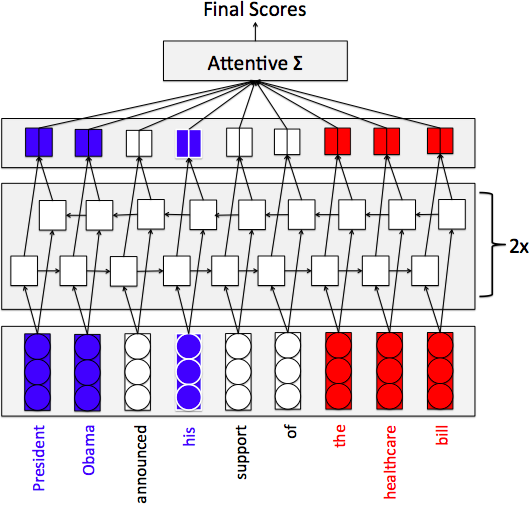
\includegraphics[scale=0.4]{base.png}
\caption{ABL architecture. Embedded tokens are passed into a 2-layer bidirectional LSTM. An attentive sum is performed over the outputs to generate final scores. In this example, \textcolor{blue}{blue} is used to represent the holder, while \textcolor{red}{red} is used to represent the target. Sample text is only one sentence, but actual documents are much longer.}
\end{figure}

\subsection{Pairwise Attentive BiLSTM (``PABL")}
\begin{figure} \label{fig:model2}
\centering
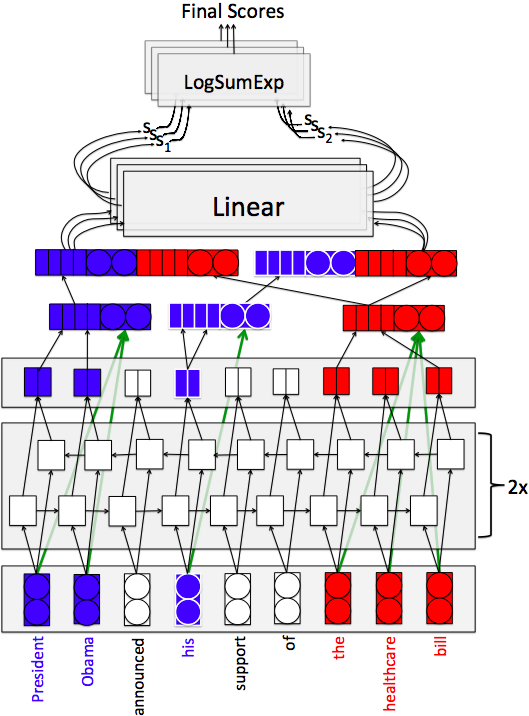
\includegraphics[scale=0.4]{adv.png}
\caption{PABL architecture. Span representations are generated by concatenating encoded start and end tokens with an attention mechanisms over embedded tokens in the span. Next, each holder span and target span are concatenated to form pairwise representations, which are fed through a linear operator to generate pairwise mention scores. Finally, mention scores are aggregated using LogSumExp.}
\end{figure}

We introduce a novel architecture for the classification of opinion sentiment.
This model is built off of ABL, with additional connections added on top.
We borrow components of this model from state-of-the-art models in relation extraction \citep{Verga:18} and co-reference resolution \citep{Lee:17}.

\noindent\textbf{Inputs.}
We concatenate two sets of embeddings to represent each token $x_t$: word embeddings ($w_t$) and polarity embeddings ($p_t$):
	$$x_t = [w_t, p_t]$$
Both embeddings are identical to those used in ABL.
Note that we do not need to append holder-target embeddings as the relation is built into the model architecture itself.

\noindent\textbf{LSTM.}
As in ABL, we use a bidirectional LSTM to contextually encode each embedded token $x_t$.
	$$x^*_t = [h_{t, 1}, h_{t, -1}]$$
% Once again, the final representation $x^*_t$ is a concatenation of the output from the forward LSTM and that from the backward LSTM.

\noindent\textbf{Span Representations.}
To represent multi-word mentions and entities (``spans"), we use span representations based on those used by \citet{Lee:17}.
For each span $i$, we take the LSTM-encoded tokens in the span and concatenate them in the following manner:
\begin{equation*}
\textbf{g}_i = [x^*_{START(i)}, x^*_{END(i)}, \hat{\textbf{x}}_i]
\end{equation*}
whereby $\textbf{x}^*_{START(i)}$ and $\textbf{x}^*_{END(i)}$ are the endpoints of the span, and $\hat{\textbf{x}}_t$ is computed using an attention mechanism over each embedded word in the span.
%The attention weights $a_{i,t}$ are computed using a feed-forward network, and normalized with softmax.
Following \citep{Lee:17}'s work, we compute the attentive representation $\hat{\textbf{x}}_i$ as a weighted sum of each embedded word $x_t$ in the span.
We make a slight modification in that we compute attention directly from the embedded token themselves, rather than deriving them from the LSTM-encoded outputs.
\begin{align*}
	\alpha_t & = \textbf{w}_\alpha \cdot FFNN_\alpha (x_t) \\
	a_{i, t} & = \frac{\exp{(\alpha_t)}}{\sum^{END(i)}_{k=START(i)} \exp{(\alpha_k)}} \\
	\hat{\textbf{x}}_i & = \sum^{END(i)}_{t = START(i)} a_{i, t}\cdot x_t
\end{align*}

\noindent\textbf{Pairwise Scoring.}
 \citet{Verga:18} scores pairs of triples using an MLP followed by a bilinear operator.
To reduce the number of parameters, we instead use a linear transformation of concatenated holder-target representations. 
We represent all combinations of the $n$ holder mentions $\textbf{g}_{1}^{holder}, \textbf{g}_{2}^{holder},\dots,\textbf{g}_{n}^{holder}$ and the $m$ target mentions $\textbf{g}_{1}^{target}, \textbf{g}_{2}^{target},\dots,\textbf{g}_{m}^{target}$ using concatenation, generating a total of $nm$ pair representations.
	$$\textbf{p}_{i, j} = [\textbf{g}_i^{holder}, \textbf{g}_j^{target}, \phi(i, j)]$$
where $\phi$ represents feature vectors for the pair $(i, j)$.
\par We then pass each pairwise representation through a linear layer. This generates scores for each (holder mention $i$, target mention $j$, sentiment $s$) triple, where $s\in\{$positive, negative, none$\}$.
	$$A_{i, j, s} = \textbf{M}\cdot \textbf{p}_{i,j}$$

\noindent\textbf{Features.}
For each holder-target mention pair, we learn separate embeddings for four different sets of features,
	$$\phi(i, j) = [\phi_s(i, j),  \phi_c(i, j), \phi_f(i, j), \phi_r(i, j)]$$
which we append to its pairwise representation $\textbf{p}_{i,j}$.
$\phi_s$ encodes how a sentence baseline model predicted the example, with different embeddings for positive, negative, and no sentiment predictions.
$\phi_c$ is a co-occurrence feature, representing the number of sentences in which the holder and target both appeared.
Finally, we have features $\phi_f$ and $\phi_r$ encoding the total number of mentions of the holder entity and target entity.
Whereas $\phi_f$ (``frequency") encodes the raw number of mentions of each entity, $\phi_r$ (``rank") encodes the ``rank" of the entity, with the most frequently mentioned entity ranked 1, the second-most frequently mentioned ranked 2, and so on.
%Importantly, note all these features remain constant for all mentions of the same entity pair.

\noindent\textbf{Aggregation.}
Our data contains labels for each entity pair, but not for each mention pair.
To deal with this, we perform multi-instance learning following \citet{Verga:18}, whereby we train the model over the aggregate of the mention pairs and perform a single update for the aggregate.
We use LogSumExp as the aggregation function. This function is a smooth approximation of the max, allowing us to extract the most probable scores for each sentiment $s$.
\begin{align*}
	score(\text{holder}, & \text{ target}, s) \\
	& = \log\sum_{\substack{i\in \{1,\dots n\},\\ j\in \{1,\dots m\}}}\exp{(A_{i, j, s})}
\end{align*}

\noindent\textbf{Training.}
We aim to maximize the log-likelihood of the correct labels for each example.
We can represent each example by the triple $(\text{document }D, \text{ holder entity }h, \text{ target entity }t)$.
\par Let $\mathcal{Y} = \{\text{Positive}, \text{ Negative}, \text{ None}\}$ represent the set of all possible labels for each example.
Given $N$ training examples labelled $y_1,\dots, y_n\in \mathcal{Y}$, with document $D$, the likelihood is given by
\begin{align*}
	P(y_1, & \dots, y_n | D, h, t) \\
	& = \prod_{i=1}^N P(y_i | D, h, t) \\
	& = \prod_{i=1}^N \frac{\exp{(score(h, t, y_i))}}{\sum_{y'\in \mathcal{Y}} \exp{(score(h, t, y'))}}
\end{align*}
We aim to maximize the the log-likelihood
	$$\sum_{i=1}^N \log{\Big(\frac{\exp{(score(h, t, y_i))}}{\sum_{y'\in \mathcal{Y}} \exp{(score(h, t, y'))}}\Big)}$$
% Probabilities here 

\noindent\textbf{Hyperparameters.}
The GloVe embeddings and learned polarity embeddings are 50-dimensional each.
All features are represent as 25-dimensional learned embeddings. The co-occurrence feature $\phi_c$ are binned into buckets: [0, 1, 2, 3, 4, 5, 6, 7, 8, 9, 10+]. The mention features $\phi_f$ and $\phi_r$ are binned into [1, 2, 3, 4, 5+].
For the biLSTM, we use 2 stacked layers and a hidden dimension of 50. We apply a dropout to the input and all hidden layers of the LSTM with probability 0.2.
For training, we optimize the model using Adam with $\alpha$ = 1e-3 and a weight decay of 1e-5. We also set $\beta_1$ = 0.9, $\beta_2$ = 0.999, $\epsilon$ = 1e-8. We use a batch size of 50 and train up to 10 epochs, with epoch 6 being selected as the optimal epoch based on development set performance.

\section{Results}
% Data statistics
\begin{table*}[!t]
\centering
\begin{tabular}{| c | r | l | l | l | l | l | l | l | l | l |}
\hline
	& & \multicolumn{3}{c |}{Neg} & \multicolumn{3}{c |}{None} & \multicolumn{3}{c |}{Pos} \\ \hline
	& & P	& R	& F1	& P	& R	& F1	& P	& R	& F1 \\ \hline
& Sentence Baseline	& 11.3	& \textbf{\underline{73.0}}	& 19.6	& 90.6	& 64.8	& 75.6	& \underline{44.8}	& 17.1	& 24.7 \\
dev- & \citet{Choi:16} SVM base	& 25.6	& 36.8	& 30.2	& 	& 	& 	& 47.3	& 36.9	& 41.4 \\
eval & \citet{Choi:16} SVM+ILP	& \textbf{37.2}	& 35.1	& 36.1	& 	& 	& 	& \bf 58.2	& 37.9	& \bf 45.9 \\
& Attentive biLSTM	& 11.8	& 59.7	& 19.9	& 90.1	& 65.8	& 76.0	& 32.5	& 19.9	& 24.7 \\
& Pairwise Attentive biLSTM	& \underline{31.9}	& 63.2	& \textbf{\underline{42.4}} & \underline{92.0}	& \underline{73.0}	& \underline{81.4}	& 30.9	& \textbf{\underline{56.7}}	& \underline{40.0} \\ \hline \hline
& Sentence Baseline	& 11.8	& \underline{\textbf{59.7}}	& 19.9	& 90.1	& 65.8	& 76.0	& \underline{32.5}	& 19.9	& 24.7 \\
test- & \citet{Choi:16} SVM base	& 27.6	& 41.2	& 33.1	& 	& 	& 	& 36.2	& 35.5	& 35.9 \\
KBP & \citet{Choi:16} SVM+ILP	& \textbf{34.6}	& 36.8	& \textbf{35.7}	& 	& 	& 	& \textbf{45.5}	& 32.7	& \textbf{38.1} \\
& Attentive biLSTM	& 19.1	& 30.4	& 23.5	& 89.6	& \underline{80.3}	& \underline{84.7}	& 29.3	& 41.8	& \underline{34.4} \\
& Pairwise Attentive biLSTM	& \underline{21.8}	& 41.6	& \underline{28.6}	& \underline{91.0}	& 69.6	& 78.9	& 23.9	& \underline{\textbf{53.2}}	& 33.0 \\ \hline \hline
& Sentence Baseline	& 10.8	& \underline{\textbf{43.8}}	& 17.4	& 89.0	& 74.1	& 80.9	& 17.5	& 3.5	& 5.9 \\
test- & \citet{Choi:16} SVM base	& \textbf{23.2}	& 16.3	& 19.2	& 	& 	& 	& \textbf{28.7}	& 23.0	& 25.6 \\
MPQA & \citet{Choi:16} SVM+ILP	& 17.6	& 24.4	& \textbf{20.4}	& 	& 	& 	& 25.2	& 29.3	& \textbf{27.1} \\
& Attentive biLSTM	& 17.9	& 23.2	& \underline{20.2}	& 88.4	& \underline{87.7}	& \underline{88.1}	& \underline{21.5}	& 17.8	& 19.4 \\
& Pairwise Attentive biLSTM	& \underline{18.8}	& 20.5	& 19.6	& \underline{89.3}	& 77.6	& 83.0	& 15.3	& \underline{\textbf{34.9}}	& \underline{21.3} \\ \hline
\end{tabular}
\caption{\label{tab:results-dev} Results on dev-eval, test-KBP, and test-MPQA. For each sentiment class, shows precision, recall, and f1 scores obtained by each model. \textbf{Bold} indicates the best score for each label among all five models, whereas \underline{underline} indicates the best score among only neural models (Sentence, Attentive biLSTM, Pairwise Attentive biLSTM). Note that \citet{Choi:16} did not report results for the `None' label.}
\end{table*}

\begin{comment}
\centering
\begin{tabular}{| l | l | l | l | l | l | l | l | l | l |}
\hline
 & \multicolumn{3}{c |}{Dev Data} & \multicolumn{3}{c |}{KBP Test Data} & \multicolumn{3}{c |}{MPQA Test Data} \\ \hline
	& P	& R	& F1	& P	& R	& F1	& P	& R	& F1 \\ \hline
Sentence	& 48.9	& 51.6	& 50.2	& 44.8	& 48.5	& 46.6	& 39.1	& 40.5	& 39.8 \\
Attentive biLSTM	& 44.8	& 48.5	& 46.6	& \textbf{46}	& 50.8	& 48.3	& \textbf{42.6}	& 42.9	& \textbf{42.8} \\
Pairwise Attentive biLSTM	 & \textbf{51.6}	& \textbf{64.3}	& \textbf{57.3}	& 45.6	& \textbf{54.8}	& \textbf{49.8}	& 41.1	& \textbf{44.3}	& 42.7 \\ \hline
\end{tabular}
\begin{table*}[!t]
\centering
\begin{tabular}{| l | l | l | l | l | l | l | l | l | l |}
\hline
ONLY POS AND NEG F1								
		Dev Data			KBP Test Data			MPQA Test Data	
	P	R	F1	P	R	F1	P	R	F1
Sentence	28.1	45.1	22.2	22.2	39.8	22.3	14.2	23.7	11.7
Pairwise	36.5	36.9	35.8	31.9	38.4	34.5	26.0	19.7	22.4
Global	47.7	36.5	41	40.1	34.8	36.9	21.4	26.9	23.8
Attentive biLSTM	22.2	39.8	22.3	24.2	36.1	29.0	19.7	20.5	19.8
Pairwise Attentive biLSTM	31.4	60.0	41.2	21.8	41.6	28.6	17.1	27.7	20.5
\hline
\end{tabular}
\end{comment}

To measure our models' performance on our task, we use precision, recall, and F1 scores.
In general, our model, which has the capacity to perform cross-sentence reasoning, performs significantly better than sentence-level baselines.
For all neural models, recall is much higher than precision if there is a sentiment (i.e. positive/negative label), while precision is much higher than recall if there is no sentiment (i.e. none label). Notably, while our F1 scores on positive and negative sentiment do not exceed that of \citet{Choi:16}, our recalls are much higher than theirs. This suggests that neural models tend to more conservative in picking ``no sentiment" labels. This additionally suggests that combining aspects of both models may be beneficial.

\subsection{Sentence Baseline}
 \citet{Socher:13} introduced a sentence-level RNN model for classifying the sentiment of sentences.
The model takes a sentence as input and classifies its sentiment into negative/neutral/positive.
We use an adaptation of this model to encapsulate how sentence-level models will perform on our task.
In our adaption, we begin by collecting all sentences in which the holder and target entities co-occur.
We then classify each of the sentences according to  \citet{Socher:13}'s model.
We classify the pair's sentiment as `none' if the entities do not co-occur in any sentence or if all sentences in which the entities co-occur in are classified as `neutral.'
We classify the pair's sentiment as `positive' if at least one sentence in which the entities co-occur in is classified as `positive.'
Otherwise, we classify the pair's sentiment as `negative.' % (if at least one sentence in which the entities co-occur is classified as `negative' or 'very negative', and no sentences are classified as `positive.')
Domain differences are the motivation for this split proportion, specifically the fact that positive labels can be up to two times more frequent than negative labels in our dataset.
\par Note that such a model assumes that any sentence in which holder and target entities co-occur express a single sentiment, and that the sentiment expressed in the sentence is the sentiment between the entity pair.
% However, these assumptions are not unreasonable, and most sentence-level approaches to fine-grained sentiment analysis also make these assumptions.
Both assumptions represent implicit limitations in sentence-level models.
Pipelined approaches to sentence-level fine-grained sentiment analysis, which first isolate sentiments before isolating the holders and targets of that sentiment \citep{Kim:2006}, also make these assumptions.
% Moreover, sentence-level models assume that entities which aren't mentioned in the same sentence do not express a sentiment, which again their inhibits performance on document-level tasks.

\subsection{SVM and SVM+ILP Baseline}
As additional baselines for comparison, we report positive and negative F1 scores from \citet{Choi:16}, which is state-of-the-art for document-level entity-entity sentiment extraction.
In \citet{Choi:16}'s SVM+ILP model, social science theories were encoded as soft ILP constraints on top of a base SVM pairwise classifier.
We report results from both the SVM base classifier and the SVM+ILP classifier with encoded constraints.
Our model, which does not use social science constraints, does not ultimately outperform the final SVM+ILP classifier.
However, it comes to within 2-3 points of the SVM base classifier.
It also has significantly higher recall than either classifier.

\subsection{Ablations on PABL}
Results from ablating our model are shown in table ~\ref{tab:ablations}.
We report performance on the development data (dev-eval) for our ablation study.
In particular, we focus on the effect of removing features.
Features for number of mentions ($\phi_f$ and $\phi_r$) contribute the most to the final results.
Mention rank features ($\phi_r$) contributed nearly 20 points to the f1 score on the negative label, and 4-7 points on none/negative labels.
Mention frequency features ($\phi_f$) contributed 11 points on the negative label and 2-4 points on none/negative labels.
This features are extremely predictive for discerning whether or not entity pairs hold sentiment, which was by far the most challenging task for the model, thus explaining why our model benefit so much from such feature.
% ^Verify this (yes, did confuse the model the most--most errors were in classifying "no sentiment" as "sentiment")
Co-occurrence features ($\phi_c$) are the next largest contributors to the final results.
This feature also helps the model determine whether sentiment is present.
Analysis on the development data shows that pairs labelled ``none"  are nearly 2 times less likely to co-occur in any sentence. Contrarily, examples labelled ``positive" and ``negative" are 2.5-3.4 times \textit{more} likely to co-occur in at least one sentence.
Finally, despite being the least helpful, sentence baseline features ($\phi_s$) still contributed 2-5 points to the f1 score.
More thorough investigations reveals that this feature boosts recall on negative examples, while boosting precision on positive examples (at the sacrifice of recall).
This trend is consistent with the performance of the sentence baseline reported in table \ref{tab:results-dev}, whereby the sentence baseline achieved the highest recall on negative examples, and the highest precision on positive examples.
\begin{table}[!t]
\centering
\begin{tabular}{| l | l | l | l |}
\hline
	& NEG	& NONE	& POS \\ \hline
PABL (Full)	& 42.4	& 81.4	& 40.0 \\
$-$ \# mentions rank $(\phi_r)$	& 22.0	& 77.2	& 33.4 \\
$-$ \# mentions $(\phi_f)$	& 33.0	& 77.7	& 38.0 \\
$-$ co-occurrence $(\phi_c)$	& 33.8	& 79.8	& 38.0 \\
$-$ sentence $(\phi_s)$	& 37.6	& 79.1	& 37.9 \\
%& \multicolumn{2}{c |}{NEG}	& \multicolumn{2}{c |}{NONE}	& \multicolumn{2}{c |}{POS} \\ \hline
%PAbL (Full)	& 42.4	& 	& 81.4	& 	& 40.0	& \\
%$-$ sentence	& 37.6	& \bf{-4.8}	& 79.1	& \bf{-2.3}	& 37.9	& \bf{-2.1} \\
%$-$ co-occurrence	& 33.8	& \bf{-8.6}	& 79.8	& \bf{-1.6}	& 38.0	& \bf{-2.0} \\
%$-$ \# mentions	& 33.0	& \bf{-9.4}	& 77.7	& \bf{-3.7}	& 38.0	& \bf{-2.0} \\
%$-$ \# mentions rank	& 22.0	& \bf{-20.4}	& 77.2	& \bf{-4.2}	& 33.4	& \bf{-6.6} \\
\hline
\end{tabular}
\caption{\label{tab:ablations} Ablations. Ablated various features and reported results on dev-eval. Each feature is important in contributing to the final F1 score.}
\end{table}


\subsection{Error Analysis of Neural Models}
We use examples from dev-eval for error analysis.
We perform error analysis on both the sentence-level baseline and our LSTM-based models to see how our models' errors compares to those made by sentence-level models, and whether it avoids the limitations posed by these models.

\noindent\textbf{Sentence Baseline.}
% Does it actually learn cross-sentence relations? (vs. something like the sentence baseline)
% how much of the errors of the sentence baseline is due to mislabelling of sentence vs. how much is due to entities which co-occur has sentence not vs. how much is due to failing to account for cross-sentence entities (i.e. mislabelling entities which do not co-occur in the same sentence) vs. how much is due to assuming sentiment of sentences entities encapsulates sentiment between entities
% now repeat for the advanced model
The most major source of error in the sentence baseline comes from misalignment between the sentiment of the sentence and the actual sentiment between entities.
We look at entity pairs which co-occurred in one sentence, since for these pairs, the sentiment of the entity pair is exactly determined by the sentiment of the sentence that they co-occur in.
Of the entity pairs which co-occur once, 87.5\% of them co-occurred in negatively-classified sentences, 4.4\% of them co-occurred in a neutral-classified sentences, and the rest co-occurred in positively-classified sentences.
However, only 7.7\% of these examples should have been labelled negatively, while as many as 73.5\% of them should have been labelled ``none."
This misalignment alone accounted for at least 72.8\%\footnote{Even this number is an underestimate as it only accounts for mistakes made by entities which co-occurred once, over the total number of mistakes.} of all mistakes made by the mode.
\par The second most common source of error is due to the model's inability to learn sentiment between sentiment pairs which do not co-occur in any sentence.
In our data, at least 23.0\% of negatively-labelled pairs and 28.0\% of positively-labelled pairs do not co-occur in a sentence.
Due to its inherent limitation as a sentence-level model, the sentence baseline is unable to classify these pairs correctly.
This accounts for 14\% of all errors.

\noindent\textbf{LSTM-Based Models: ABL and PABL.} % Rename this
As observed, one limitation of the sentence baseline is its inability to classify non-co-occurring pairs as holding sentiment.
On the other hand, LSTM-based models do actually learn to classify non-co-occurring as positive or negative.
In fact, these models have the opposite problem of being over-zealous in doing so, with 39\% of its predicted negative pairs and 35\% of its predicted positive pairs not co-occurring in any sentence.
In actuality, only 23\% of negative pairs and 28\% of positive pairs do not co-occur in any sentence.
This mirrors the larger trend whereby LSTM-based models are overeager in predicting pairs as holding sentiment 
\par Incorrectly classifying ``none" examples as either ``positive" or ``negative" accounted for 62.8\% and 81.5\% of all errors respectively, for both the ABL and PABL model.
This trend is shown in table \ref{tab:breakdown}.
This is also consistent with the precision/recall scores for each label as reported in table \ref{tab:results-dev}, with recall being much higher than precision for positive and negative examples, and precision being higher than recall for ``none" examples.
\par The annotations themselves may contribute to the model's poor performance in identifying ``none" examples.
``None" examples are by far the most difficult and subjective label to annotate.
As an example, different documents containing the phrase ``[Country] President [Person]" were annotated differently.
In some documents, holder = [Person], target = [Country] was labelled ``positive," whereas in others (such as the document in the introduction) holder = [Person], target = [Country] was labelled ``none."
These inconsistent annotations, especially on ``none" examples, can harm the performance of our model.
\par Surprisingly, the vanilla version of the pairwise attentive bidirectional LSTM without any features does not outperform the attentive bidirectional LSTM.
However, with the addition of features, this model receives a significant boost in performance.
% Table showing breakdown of labels & how they were predicted. By far largest mistake is no sentiment/sentiment
\begin{table}[!t]
\centering
\begin{tabular}{| l | l | l  l  l |}
\hline
	& 	& 	\multicolumn{3}{c |}{Label} \\ \hline
	& 	& Neg	& None	& Pos \\ \hline
ABL	& Neg	& \bf 84	& 213	& 66 \\
Pred-	& None	& 52	& \bf 1946	& 145 \\
iction	& Pos	& 38	& 295	& \bf 193 \\ \hline \hline
PABL	& Neg	& \bf 130	& 332	& 94 \\
Pred-	& None	& 29	& \bf 1487	& 82 \\
iction	& Pos	& 15	& 635	& \bf 228 \\
\hline
\end{tabular}
\caption{\label{tab:breakdown} Model predictions vs. actual classifications of example for both LSTM-based models. \textbf{Bold} is used to signify the most frequent prediction for each label. The most significant source of error for both models is the classification of ``none" examples as ``neg" or ``pos." This is especially apparent for PABL.}
\end{table}

\section{Related Work}
Very little research has been done thus far on document-level extraction of entity-to-entity sentiment relations.
Of what has been done, \citet{Choi:16} uses a SVM-based model to predict directed opinions in text, and investigates the effect of encoding social science theories into their model.
Our work uses neural models, which require less features and thus less preprocessing.
\par Related work in fine-grained sentiment analysis usually
%, a task involving identification of sentiment polarity, holder, and/or target,
focuses on one or more aspects of the task, such as identifying sentiment expression \citep{Irsoy:14}, identifying sentiment target \citep{Liu:15}, jointly extracting sentiment polarity and target \citep{Mitchell:13}, or jointly extracting sentiment polarity, holder, and target \citep{Katiyar:16, Yang:13}.
The latter two tasks require combining sentiment analysis with NER.
In this work we focus solely on classifying sentiment polarity.
\par Popular approaches to fine-grained sentiment analysis include CRFs \citep{Yang:12, Mitchell:13} and CRF+ILP joint models \citep{Yang:13}.
More recently, recurrent neural networks, in particular LSTMs, have proven to be effective for this task \citep{Liu:15, Irsoy:14}.
There is some conflicting literature in regards to how LSTMs perform relative to CRFs.
\citet{Irsoy:14} finds that multi-layer bi-directional LSTMs outperform CRFs on opinion expression extraction, and \citet{Liu:15} finds that LSTMs used in conjugation with word embeddings outperform CRFs on opinion target extraction without the need for feature engineering.
On the other hand, \citet{Katiyar:16} finds that bi-directional LSTMs do not outperform conventional CRFs for holder and target extraction, but that adding sentence-level and relation-level dependencies to the final layer improves performance to within 1-3\% of CRF models.
Almost all models in this field operate on the sentence level, where one sentiment is being expressed between one holder and one target.
Our work differs by working at the document level, focused on capturing complex networks of sentiments between many different entity pairs.
\par Our pairwise attentive biLSTM model borrows architectural components from related fields such as co-reference resolution and document-level relation extraction.
We represent mention spans by concatenating encoded start and end tokens with an attentive mechanism.
These span representations have been used with relative success in co-reference resolution \citep{Lee:17}, with the attention component shown to be particularly useful.
The generation of pairwise scores between all mentions of each entity and the use of the LogSumExp aggregation function over these scores were inspired by techniques used in document-level relation extraction, in particular the model introduced by \citet{Verga:18}.

\section{Conclusion}
We present two LSTM-based neural models for document-level entity-entity sentiment analysis. Both models significantly outperform the sentence-level baseline.
We find that the sentence-level model performs poorly on this task, suggesting that current research in intra-sentence sentiment analysis may not generalize to document-level texts.
We additionally find that LSTM-based models may not perform as well as state-of-the-art SVM models.
Neural models are generally overeager in assigning sentiment between entity pairs, producing overly dense sentiment networks for each document.
\par In the future, we hope to explore means to strategically prune excess sentiment relations.
We would also like to explore encoding social science constraints into our model, either by encoding the constraints in the loss function while training or by designing an architecture to explicitly model the constraints.
Finally, joint extraction of sentiment polarities, holders, and/or targets, have proven to outperform pipelined approached to fine-grained sentiment analysis \citep{Yang:13}.
These are all directions to explore in future work.
% which have proven to be helpful , are.
% These are all directions for future work.

\section*{Acknowledgments}
I would like to thank Eunsol Choi for her invaluable contributions to this work.
I would also like to thank Yejin Choi, Ari Holtzmann, and Nelson Liu for their advice and feedback.

\bibliographystyle{./acl_natbib_nourl}
\bibliography{./emnlp2018}

\appendix

\end{document}
